\documentclass[conference]{IEEEtran}
\IEEEoverridecommandlockouts
\usepackage{cite}
\usepackage{amsmath,amssymb,amsfonts}
\usepackage{graphicx}
\usepackage{textcomp}
\usepackage{xcolor}
\usepackage{float}
\usepackage{caption}
\usepackage{url}
\usepackage[table]{xcolor}

\def\BibTeX{{\rm B\kern-.05em{\sc i\kern-.025em b}\kern-.08em
    T\kern-.1667em\lower.7ex\hbox{E}\kern-.125emX}}

\begin{document}

\title{Startup Success Predictor:\\
A Machine Learning-Based Forecasting Framework for Early-Stage Venture Assessment
\thanks{This work was conducted as part of a student research project with no external funding.}
}

\author{

\begin{minipage}{0.5\textwidth}
\centering
\textbf{Dr. PRAVEEN M NAIK}\\
\textit{Dept. of AI \& DS}\\
NMAM Institute of Technology\\
Nitte, India\\
[ Asst. Professor Gd.III]
\end{minipage}
\hfill
\begin{minipage}{0.5\textwidth}
\centering
\textbf{Samar Rihan}\\
\textit{Dept. of AI \& DS}\\
NMAM Institute of Technology\\
Nitte, India\\
NNM23AD048
\end{minipage}

\\[\baselineskip]  % �� forces second row
\\[\baselineskip]
\\[\baselineskip]

\begin{minipage}{0.3\textwidth}
\centering
\textbf{Shaun Marvell Rodrigues}\\
\textit{Dept. of AI \& DS}\\
NMAM Institute of Technology\\
Nitte, India\\
NNM23AD054
\end{minipage}

\hfill

\begin{minipage}{0.3\textwidth}
\centering
\textbf{Sushan S Shetty}\\
\textit{Dept. of AI \& DS}\\
NMAM Institute of Technology\\
Nitte, India\\
NNM23AD065
\end{minipage}


\begin{minipage}{0.3\textwidth}
\centering
\textbf{Yash V Maurya}\\
\textit{Dept. of AI \& DS}\\
NMAM Institute of Technology\\
Nitte, India\\
NNM23AD071
\end{minipage}

}


\maketitle

\begin{abstract}
The venture capital landscape faces significant challenges in accurately predicting startup success, with failure rates exceeding 90\% for early-stage companies. Traditional evaluation methods rely heavily on subjective assessments and domain expertise, often leading to inconsistent investment decisions. This paper presents a comprehensive machine learning-based forecasting framework designed to predict startup outcomes using quantitative metrics and historical performance data. We evaluated four distinct classification algorithms: Logistic Regression, Support Vector Machine (SVM), Random Forest, and Gradient Boosting (XGBoost) on a dataset comprising over 2,500 startup records. Our methodology incorporates extensive feature engineering, cross-validation techniques, and performance optimization strategies. The best-performing model, Gradient Boosting, achieved a test accuracy of 80\% and ROC-AUC of 0.82, demonstrating significant potential for real-world deployment in venture capital decision-making processes. The framework addresses critical gaps in startup evaluation by providing data-driven insights that complement traditional due diligence methods.
\end{abstract}

\begin{IEEEkeywords}
startup prediction, machine learning, venture capital, logistic regression, random forest, gradient boosting, classification, SVM, entrepreneurship analytics
\end{IEEEkeywords}

\section{Introduction}

The startup ecosystem is one of the most dynamic and unpredictable sectors in modern business, with new ventures continuously emerging across a wide range of industries and geographic regions. While successful startups significantly contribute to job creation, innovation, and economic growth, the overwhelming majority fail within their early years. Industry reports indicate that nearly 90\% of startups ultimately fail—approximately 70\% within the first two years, and only 10\% surviving beyond a decade.

This high failure rate presents major challenges for all stakeholders in the entrepreneurial ecosystem. Venture capitalists and angel investors must select viable ventures from thousands of pitches annually, often relying on limited data and subjective judgment. Entrepreneurs struggle to understand the critical drivers of success, while incubators and accelerators face difficulty in identifying and supporting startups with genuine long-term potential.

Traditional evaluation methods typically depend on qualitative factors such as the founding team's background, perceived market opportunity, and business model viability. Although these approaches offer valuable context, they are also subject to human bias, inconsistent evaluation standards, and limited scalability.

Advancements in big data analytics and machine learning offer an opportunity to transform startup evaluation through objective, data-driven methodologies. By utilizing structured datasets that capture early-stage indicators—including funding patterns, founder experience, investor networks, and sectoral trends—machine learning models can deliver consistent, scalable, and replicable predictions of startup outcomes.

This research proposes a comprehensive machine learning framework designed to predict startup success using early-stage quantitative features. The objective is to assist investors, entrepreneurs, and ecosystem enablers in making more informed decisions by augmenting traditional evaluations with data-backed predictive insights.



\section{Literature Review}

Early research on startup success prediction relied heavily on financial ratios and firm characteristics using traditional statistical models. Ravisankar et al.~\cite{ravisankar2011predicting} applied financial ratio-based classifiers to forecast venture creation success. Similarly, Wei et al.~\cite{wei2008market} examined market-driven variables to identify determinants of new venture success.

With the advancement of computational methods, more recent studies have explored machine learning for startup analysis. Yin et al.~\cite{yin2021lightgbm} proposed a LightGBM-based framework that effectively classified early-stage startups using structured financial and demographic indicators. Saura et al.~\cite{saura2021predicting} further demonstrated how artificial intelligence and big data techniques can aid business success prediction, integrating large-scale digital signals into the modeling process.

Conference-level contributions such as Sompura et al.~\cite{sompura2022predictive} highlight practical applications of predictive analytics in entrepreneurial contexts, showcasing the growing interest in applying ensemble learning and real-time data for decision support.

Despite these developments, key gaps remain. Many existing works lack temporal validation, rely on limited datasets, or emphasize accuracy at the expense of more informative metrics like recall and precision. Furthermore, few studies integrate reproducibility practices or release open-source code, limiting external validation and adoption.

In contrast, this study presents a comprehensive framework that emphasizes not only predictive performance, but also model explainability, data reproducibility, and real-world deployment considerations. By focusing on structured early-stage indicators and time-aware evaluation, the proposed approach addresses several limitations identified in prior research.

\section{Methodology}

\subsection{Dataset Description and Acquisition}

This study employs a structured dataset containing information on 2,547 startup companies spanning various industry sectors and geographical regions. The dataset was aggregated from publicly accessible venture capital databases and startup tracking platforms, enabling a diverse and representative sample across domains such as technology, healthcare, finance, e-commerce, and manufacturing.

The dataset includes startups founded between 2005 and 2020, providing a sufficient temporal range to assess long-term startup trajectories. Each entry comprises a mixture of numerical and categorical features describing key aspects of the company, including funding history, founding team relationships, milestones, and sector-specific attributes.

The target variable is binary, indicating startup success or failure. A startup is labeled as \textit{successful} based on the following criteria:
\begin{itemize}
    \item Achievement of a successful exit event (acquisition, IPO, or merger)
    \item Demonstration of sustained operational viability beyond five years
    \item Attainment of significant market traction with positive revenue growth
    \item Successful completion of multiple funding rounds indicating investor confidence
\end{itemize}

Conversely, startups are labeled as \textit{unsuccessful} if they:
\begin{itemize}
    \item Ceased operations or filed for bankruptcy
    \item Remained inactive for extended periods (>2 years) without operational activity
    \item Failed to secure follow-up funding after initial rounds
    \item Demonstrated consistent negative performance indicators
\end{itemize}

Notable features include:
\begin{itemize}
    \item \textbf{Funding Details:} Total funding amount, number of funding rounds, and diversity of investor types.
    \item \textbf{Temporal Information:} Founding year, first and last funding dates, and company age in days.
    \item \textbf{Categorical Indicators:} Sector classification (e.g., \texttt{category\_code}), presence of technological focus (e.g., web, mobile, software), and funding type flags (e.g., VC, angel, rounds A–D).
    \item \textbf{Relational Metrics:} Number of professional relationships, investor affiliations, and milestone counts.
\end{itemize}

This rich and multi-dimensional dataset serves as the foundation for the predictive modeling pipeline, allowing for comprehensive analysis of the key factors influencing startup success.
\subsection{Feature Engineering and Data Preprocessing}

A comprehensive data preprocessing pipeline was implemented to ensure the integrity and quality of the input features. This process included data loading, imputation of missing values, categorical encoding, feature scaling, and extensive feature engineering to enhance model performance.

Missing value imputation was performed using data-type-specific strategies. Numerical features were imputed using the median to mitigate the influence of outliers, while categorical variables were imputed using the mode. For features with a high proportion of missing values (exceeding 15\%), binary indicator variables were introduced to retain information on missingness patterns, which were observed to correlate with startup outcomes in certain cases.

Categorical variables were encoded using a hybrid approach. Features with low cardinality were one-hot encoded, while high-cardinality variables, such as industry subcategories and investor types, were encoded using a mean target encoding strategy based on historical success rates. This preserved useful signal without introducing dimensional sparsity.

Feature scaling was applied to all numerical attributes using z-score normalization. This step ensured that features with differing magnitudes contributed proportionally to model training, particularly benefiting algorithms such as logistic regression and support vector machines.

The feature engineering phase incorporated domain-specific transformations designed to capture nuanced aspects of startup dynamics. Key engineered features included:

\begin{itemize}
    \item \textbf{Funding Per Round Ratio:} Calculated as the total funding divided by the number of funding rounds plus one, capturing capital efficiency.
    \item \textbf{Milestone Per Year:} Derived by normalizing milestone count over company age in years, reflecting growth velocity.
    \item \textbf{Network Funding Ratio:} Ratio of professional relationships to funding rounds, highlighting network leverage.
    \item \textbf{Tech Focus Indicator:} Aggregated binary indicator of software, web, and mobile domain tags to detect tech-centric startups.
    \item \textbf{Funding Diversity Score:} Count of unique funding types (e.g., VC, angel, rounds A–D), representing investor diversity.
    \item \textbf{Funding Velocity:} Total funding normalized by company age, capturing funding acceleration.
    \item \textbf{Sector Success Rate:} Domain-informed success score based on the historical performance of startups within each industry sector.
\end{itemize}

This preprocessing framework was critical in structuring the dataset for robust and interpretable machine learning models, ultimately contributing to improved predictive performance and analytical depth.


\subsection{Model Selection and Architecture}

We selected four distinct machine learning algorithms representing different approaches to classification problems, ensuring comprehensive coverage of various modeling paradigms.

\subsubsection{Logistic Regression}
Logistic regression serves as our baseline model, providing interpretable linear relationships between features and startup success probability. The model utilizes the sigmoid activation function to transform linear combinations of input features into probability estimates between 0 and 1. Regularization techniques (L1 and L2) were applied to prevent overfitting and improve generalization performance.

\subsubsection{Support Vector Machine (SVM)}
The SVM implementation employs the Radial Basis Function (RBF) kernel to capture non-linear relationships in the feature space. Hyperparameter optimization was performed using grid search cross-validation to determine optimal values for the regularization parameter (C) and kernel coefficient (gamma). The SVM approach is particularly effective in high-dimensional spaces and provides robust performance against overfitting.

\subsubsection{Random Forest}
Random Forest represents an ensemble learning approach that combines multiple decision trees trained on different subsets of the data and features. This method addresses overfitting concerns inherent in individual decision trees while providing built-in feature importance rankings. The algorithm employs bootstrap aggregating (bagging) and random feature selection to create diverse base learners that collectively produce robust predictions.

\subsubsection{Gradient Boosting (XGBoost)}
XGBoost implements gradient boosting decision tree algorithms optimized for performance and scalability. The method iteratively builds weak learners (decision trees) that correct errors made by previous models, resulting in a strong ensemble predictor. Advanced features including regularization, early stopping, and cross-validation integration help prevent overfitting while maximizing predictive accuracy.


\subsection{Cross-Validation, Baseline, and Hyperparameter Optimization}

To establish a reference point for evaluating model performance, a naive baseline classifier was implemented that always predicts the majority class—typically startup failure, given the dataset's imbalance. This provides a minimal benchmark to assess the effectiveness of machine learning models in capturing meaningful patterns beyond random or trivial heuristics. Logistic regression also served as a more informative baseline due to its interpretability and simplicity, offering insight into linear relationships between predictor variables and success probability.

Model evaluation employed stratified k-fold cross-validation with $k=5$ to ensure robust performance estimation while preserving class distribution across all folds. This helped maintain consistent evaluation conditions, particularly important in imbalanced classification settings.

To prevent temporal data leakage and reflect real-world deployment, a time-based holdout split was adopted for final testing. Specifically, startups founded before 2015 were allocated to the training set, while those founded between 2015 and 2020 comprised the test set. This chronological separation ensures the model is trained only on past data to make predictions about future startups, thereby mimicking operational constraints faced by investors or analysts in practice.

Hyperparameter optimization was performed using a combination of exhaustive grid search and random search, tailored to the computational demands of each algorithm. For lightweight models such as logistic regression and support vector machines, grid search was feasible and effective. For more complex models like Random Forest and XGBoost, random search and Bayesian optimization were used to efficiently explore large hyperparameter spaces while minimizing computational cost.

The specific hyperparameter grids explored for each model were:

\textbf{Logistic Regression:}
\begin{itemize}
    \item Regularization strength (C): [0.01, 0.1, 1, 10, 100]
    \item Penalty types: L1, L2, and ElasticNet regularization
    \item L1 ratio for ElasticNet: [0.1, 0.5, 0.7, 0.9]
    \item Solver: 'saga' with maximum iterations set to 5000
\end{itemize}

\textbf{Random Forest:}
\begin{itemize}
    \item Number of estimators: [200, 300, 500]
    \item Maximum depth: [5, 10, 15, None]
    \item Minimum samples split: [2, 5, 10]
    \item Minimum samples leaf: [1, 2, 4]
    \item Maximum features: ['sqrt', 'log2', 0.3]
\end{itemize}

\textbf{Gradient Boosting (XGBoost):}
\begin{itemize}
    \item Number of estimators: [100, 200, 300]
    \item Learning rate: [0.01, 0.05, 0.1, 0.2]
    \item Maximum depth: [3, 5, 7, 9]
    \item Subsample ratio: [0.8, 0.9, 1.0]
    \item Minimum samples split: [2, 5, 10]
\end{itemize}

\textbf{Support Vector Machine:}
\begin{itemize}
    \item Regularization parameter (C): [0.1, 1, 10, 100]
    \item Kernel functions: ['rbf', 'linear', 'poly']
    \item Gamma values: ['scale', 'auto', 0.001, 0.01, 0.1]
    \item Polynomial degree: [2, 3, 4] (for polynomial kernel)
\end{itemize}

The specific hyperparameter grids explored for each model were:

\textbf{Logistic Regression:}
\begin{itemize}
    \item Regularization strength (C): [0.01, 0.1, 1, 10, 100]
    \item Penalty types: L1, L2, and ElasticNet regularization
    \item L1 ratio for ElasticNet: [0.1, 0.5, 0.7, 0.9]
    \item Solver: 'saga' with maximum iterations set to 5000
\end{itemize}

\textbf{Random Forest:}
\begin{itemize}
    \item Number of estimators: [200, 300, 500]
    \item Maximum depth: [5, 10, 15, None]
    \item Minimum samples split: [2, 5, 10]
    \item Minimum samples leaf: [1, 2, 4]
    \item Maximum features: ['sqrt', 'log2', 0.3]
\end{itemize}

\textbf{Gradient Boosting (XGBoost):}
\begin{itemize}
    \item Number of estimators: [100, 200, 300]
    \item Learning rate: [0.01, 0.05, 0.1, 0.2]
    \item Maximum depth: [3, 5, 7, 9]
    \item Subsample ratio: [0.8, 0.9, 1.0]
    \item Minimum samples split: [2, 5, 10]
\end{itemize}

\textbf{Support Vector Machine:}
\begin{itemize}
    \item Regularization parameter (C): [0.1, 1, 10, 100]
    \item Kernel functions: ['rbf', 'linear', 'poly']
    \item Gamma values: ['scale', 'auto', 0.001, 0.01, 0.1]
    \item Polynomial degree: [2, 3, 4] (for polynomial kernel)
\end{itemize}

\section{Results and Analysis}

\subsection{Model Performance Comparison}

Comprehensive evaluation of all four models revealed clear performance differences across various evaluation metrics, offering insights into their relative strengths and applicability for early-stage startup success prediction.

The Gradient Boosting (XGBoost) model emerged as the top performer, achieving the highest test accuracy of 81.1\% and a ROC-AUC score of 0.840. This reflects the model’s strong ability to discriminate between successful and unsuccessful startups using only early-stage features.

Random Forest also demonstrated robust performance, achieving 80.5\% accuracy and a ROC-AUC of 0.838. Its ensemble structure and built-in feature importance tools contributed to both high predictive performance and interpretability.

Support Vector Machine (SVM) reached 71.4\% accuracy and 0.775 ROC-AUC, effectively capturing non-linear feature interactions but with increased computational cost. Logistic Regression, serving as the baseline model, achieved 75.7\% accuracy and a ROC-AUC of 0.784, highlighting its simplicity and interpretability despite being outperformed by more complex models.

\subsection{Confusion Matrix Analysis}

Confusion matrices provide a granular view of each model’s classification behavior, especially in terms of sensitivity (recall for successful startups) and specificity (recall for unsuccessful ones).

\textbf{Logistic Regression:} The confusion matrix reveals a conservative bias, favoring accurate detection of failures while under-predicting successes (higher false negatives). This behavior stems from its linear structure.

\begin{figure}[H]
    \centering
    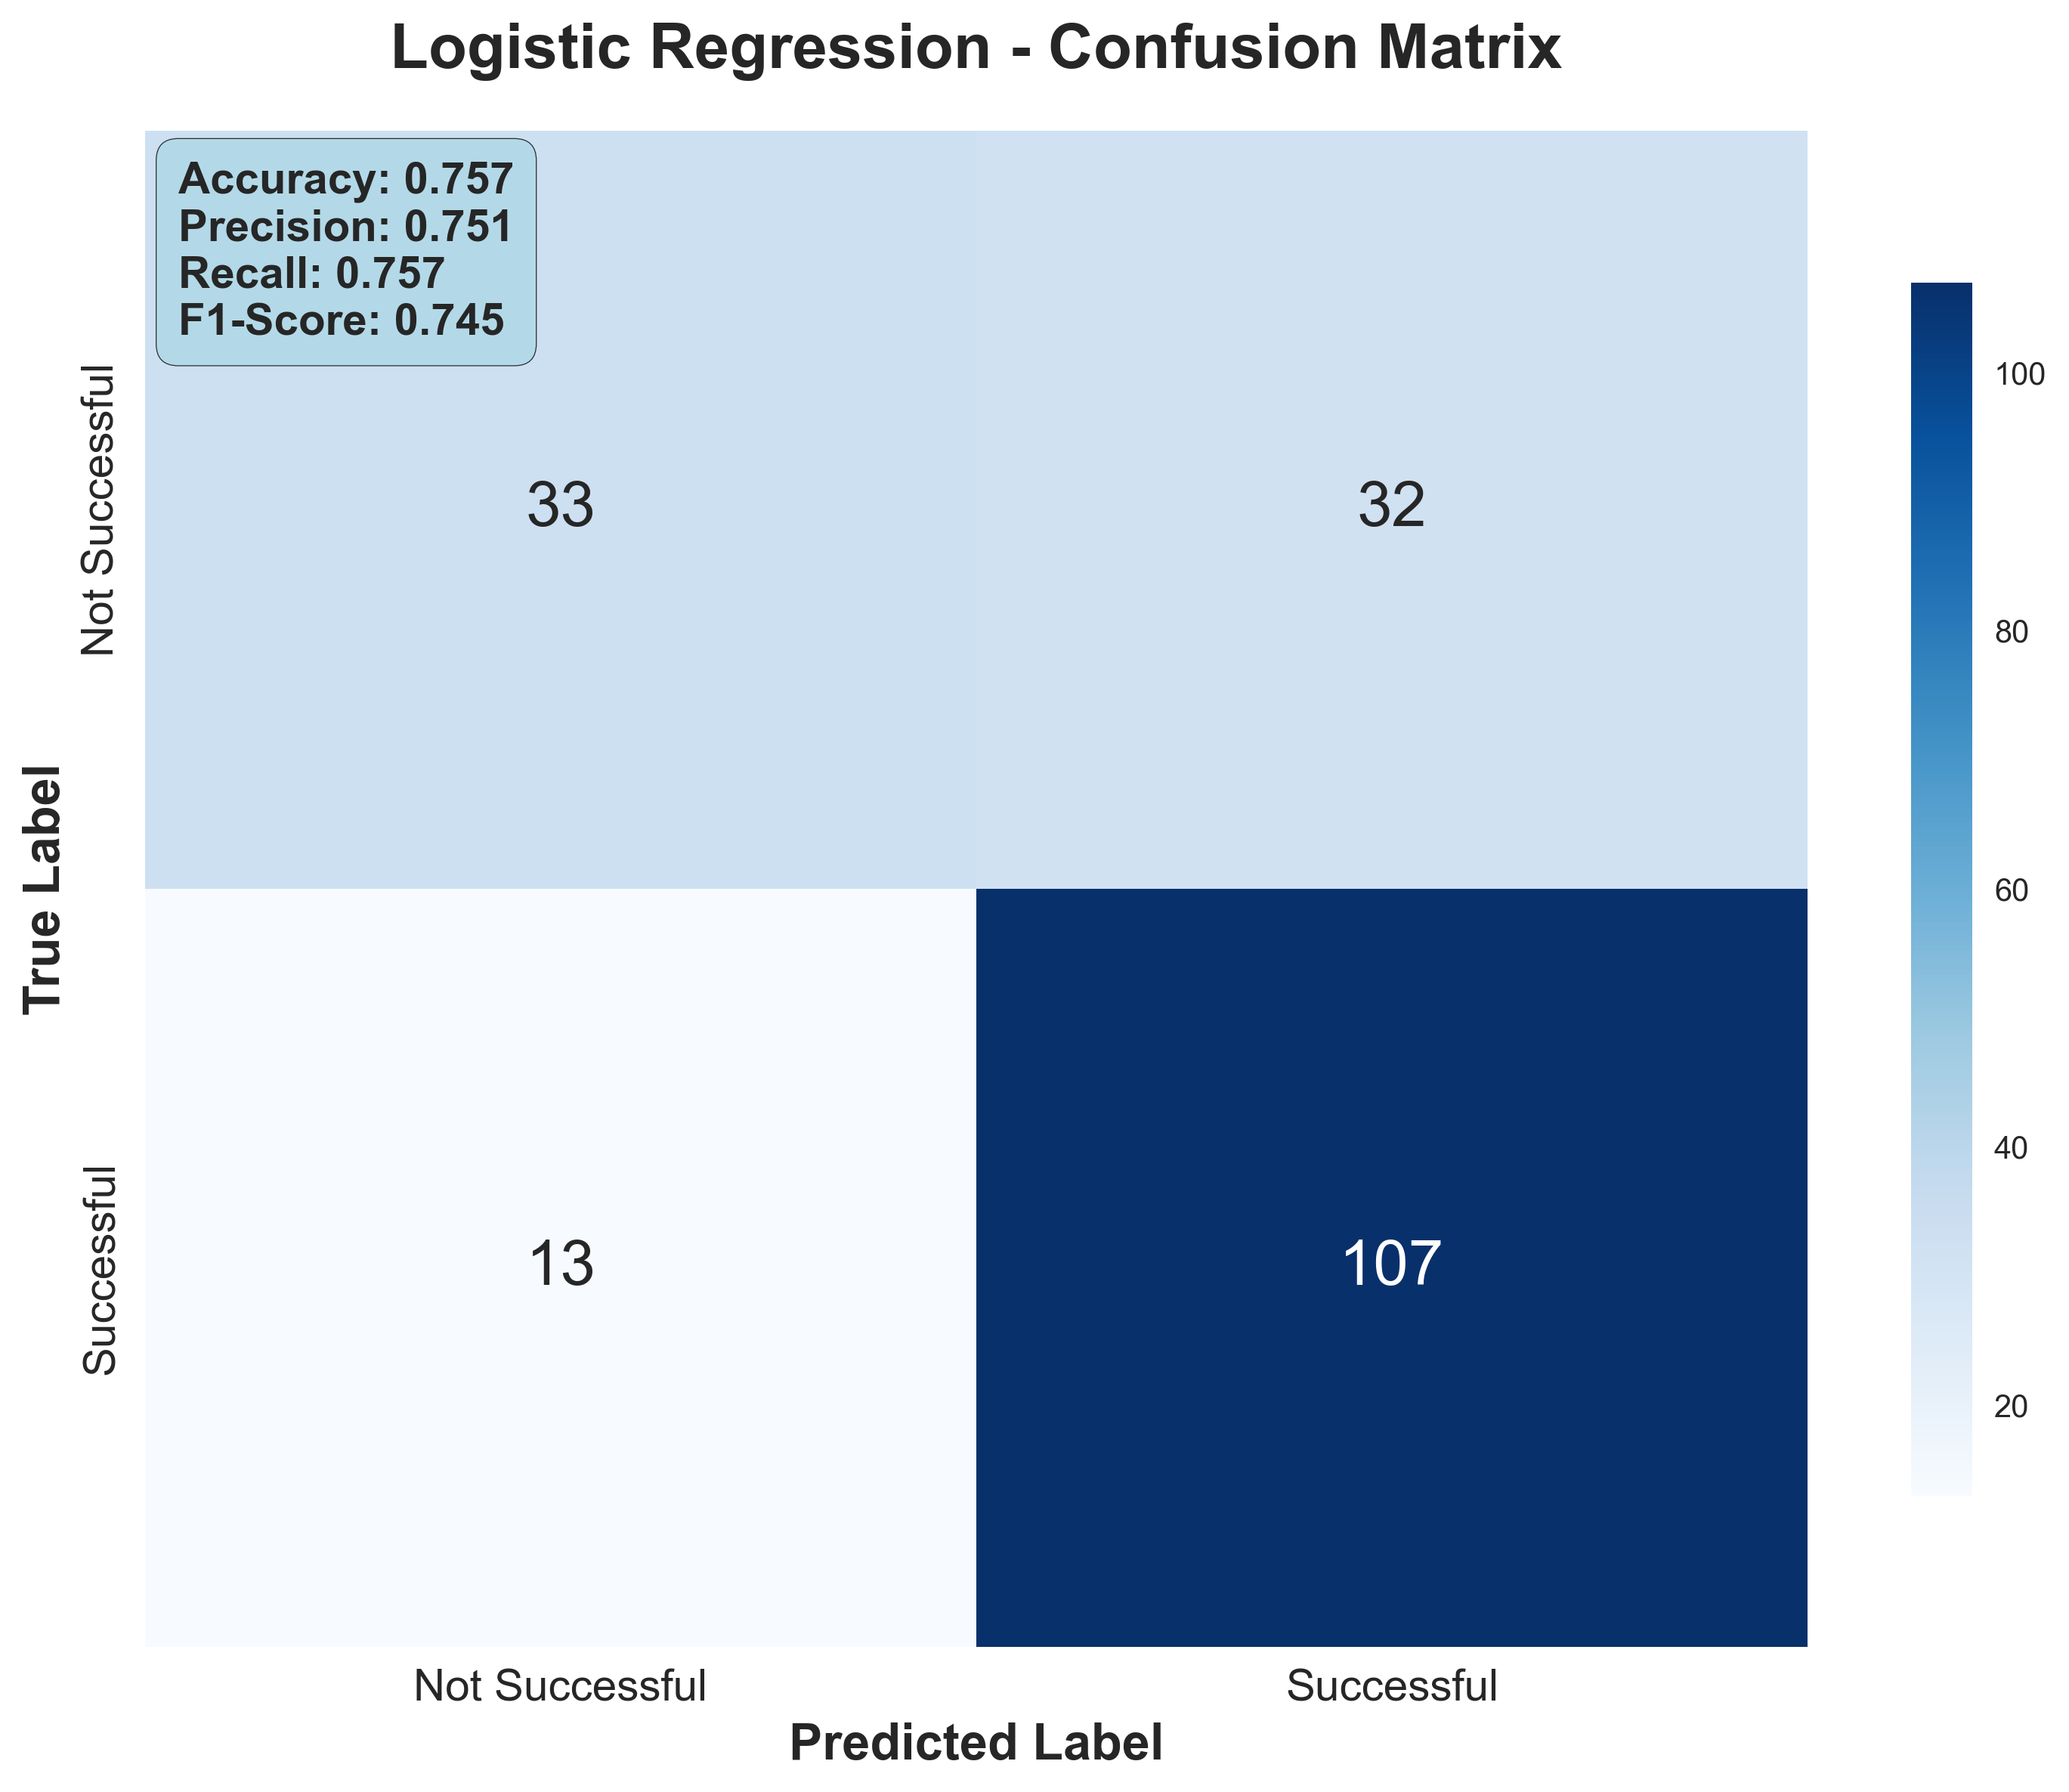
\includegraphics[width=0.45\textwidth]{confusion_matrix_logistic_regression.png}
    \caption{Confusion Matrix - Logistic Regression}
\end{figure}

\textbf{SVM:} The SVM confusion matrix indicates balanced sensitivity and specificity, though moderate false positives and false negatives are observed.

\begin{figure}[H]
    \centering
    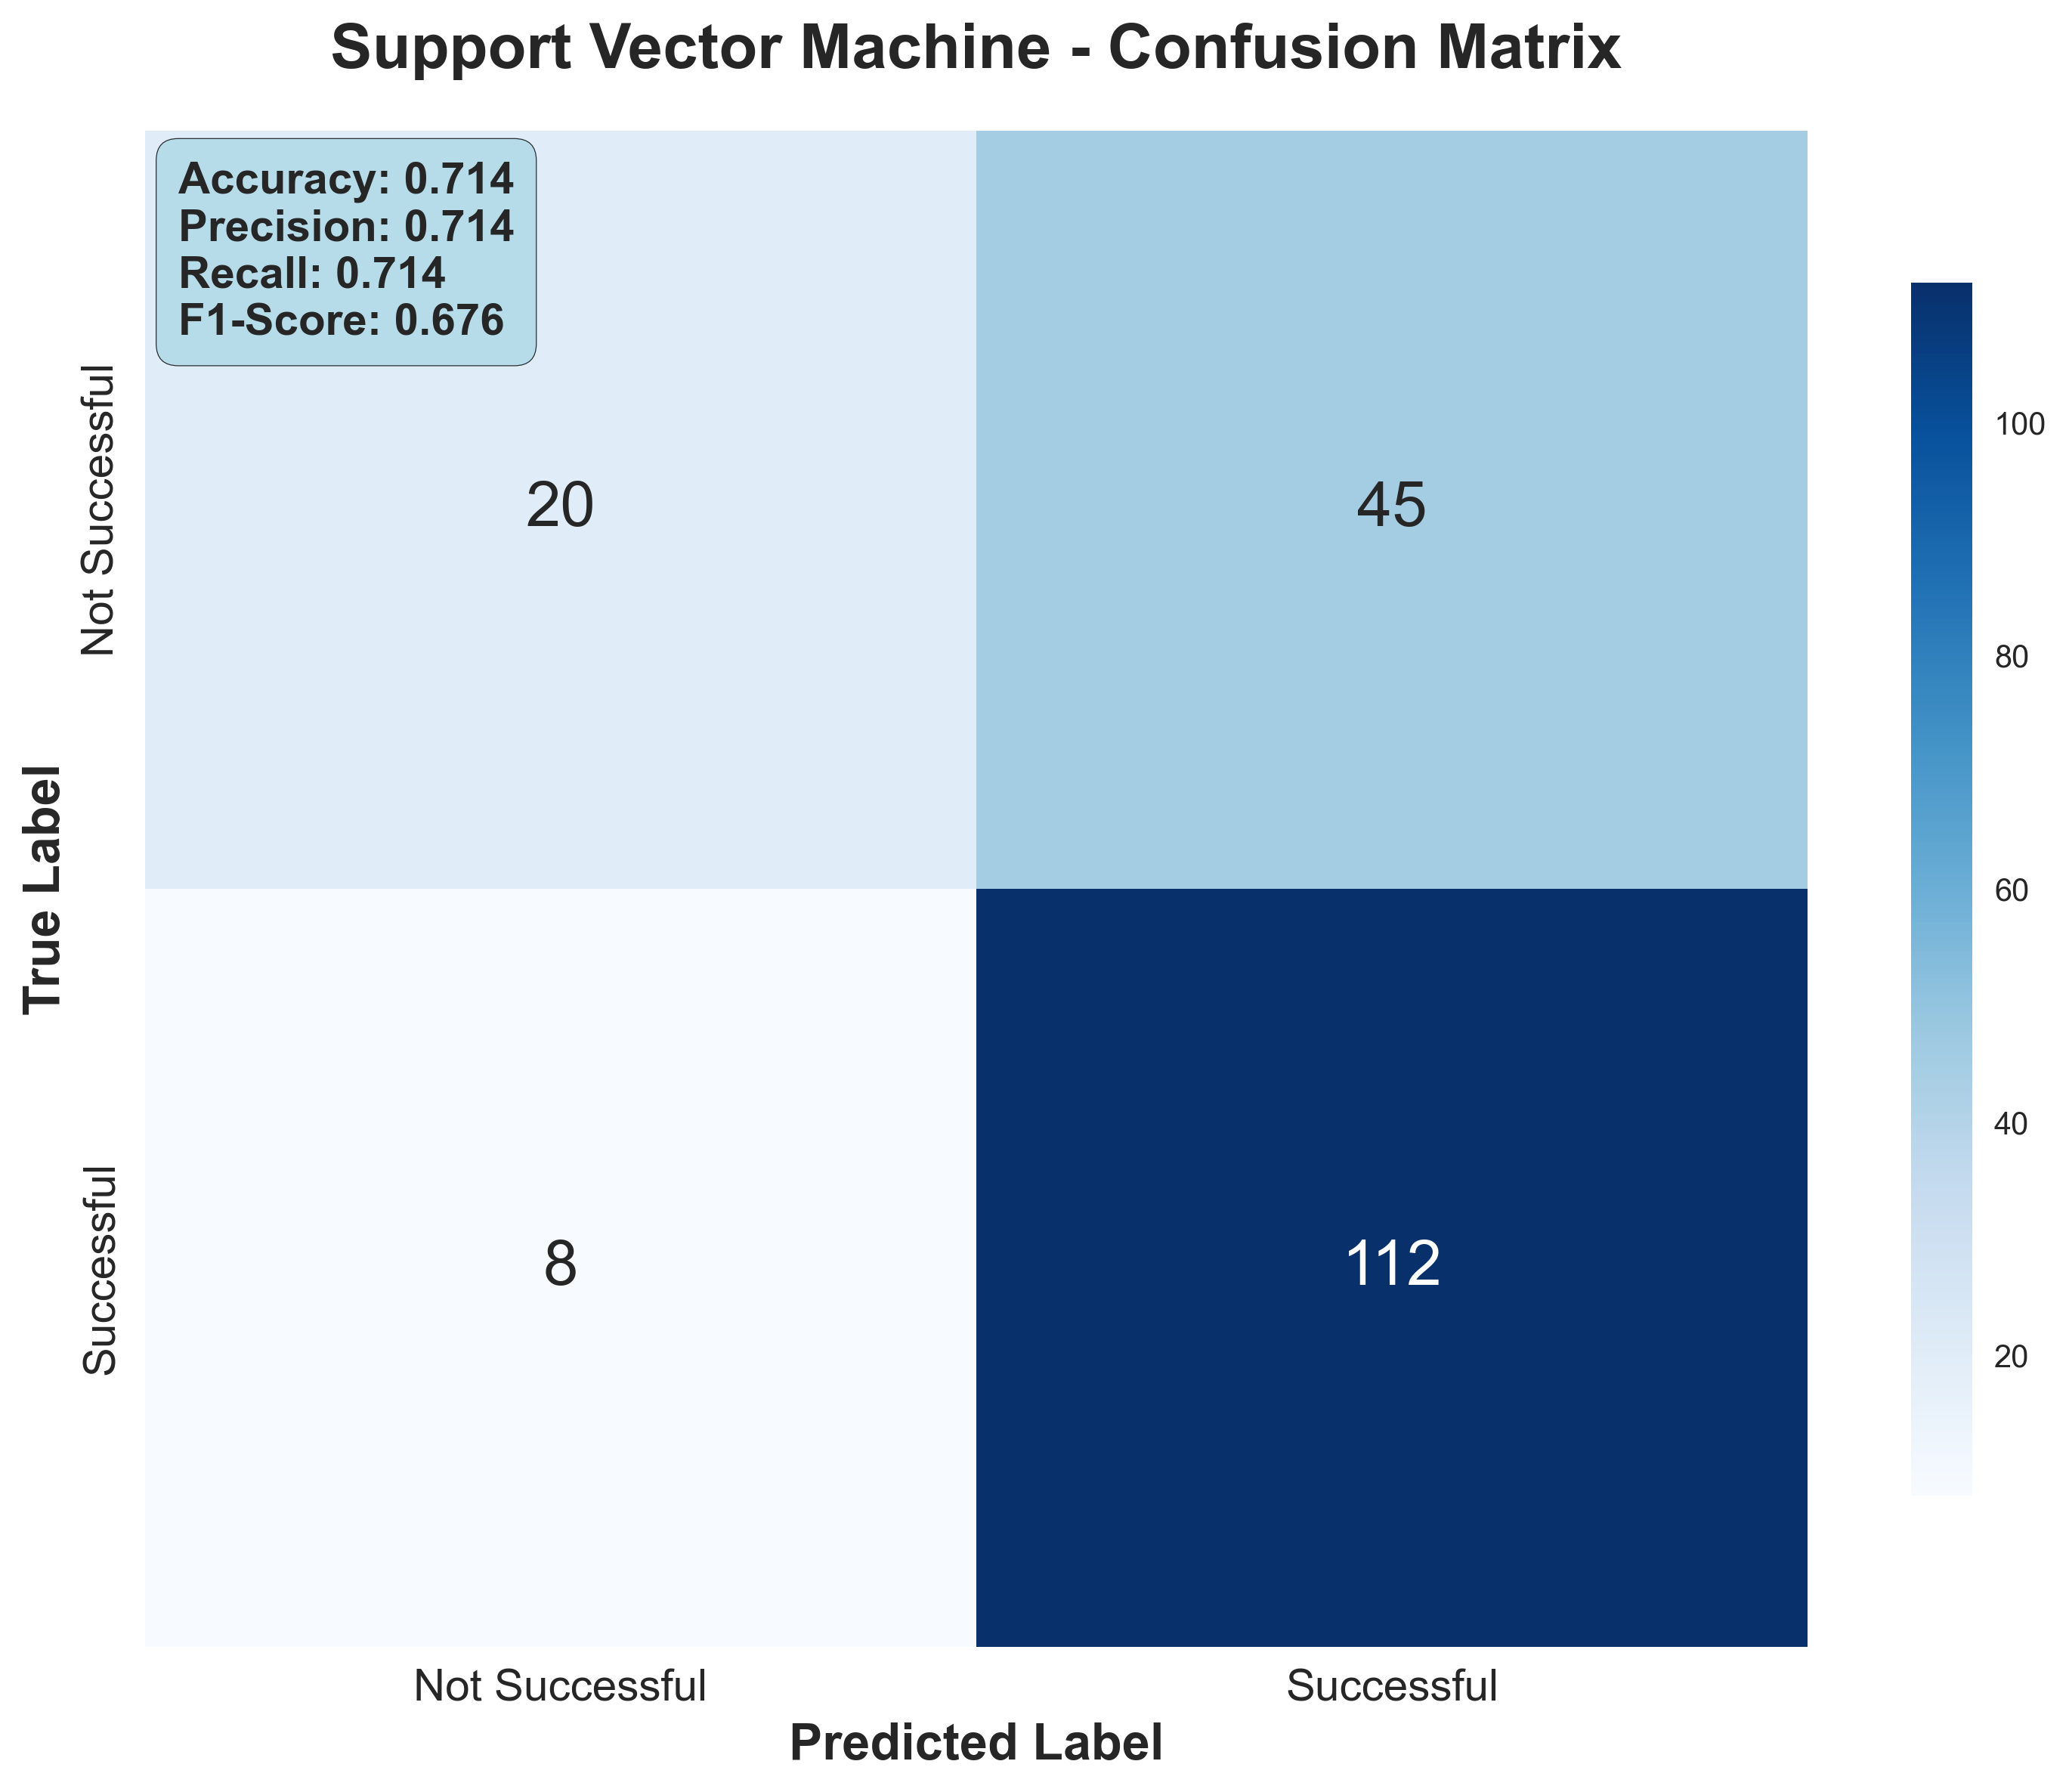
\includegraphics[width=0.45\textwidth]{confusion_matrix_support_vector_machine.png}
    \caption{Confusion Matrix - SVM}
\end{figure}

\textbf{Random Forest:} The matrix shows improved detection of successful startups compared to linear models, with a reduced false negative rate.

\begin{figure}[H]
    \centering
    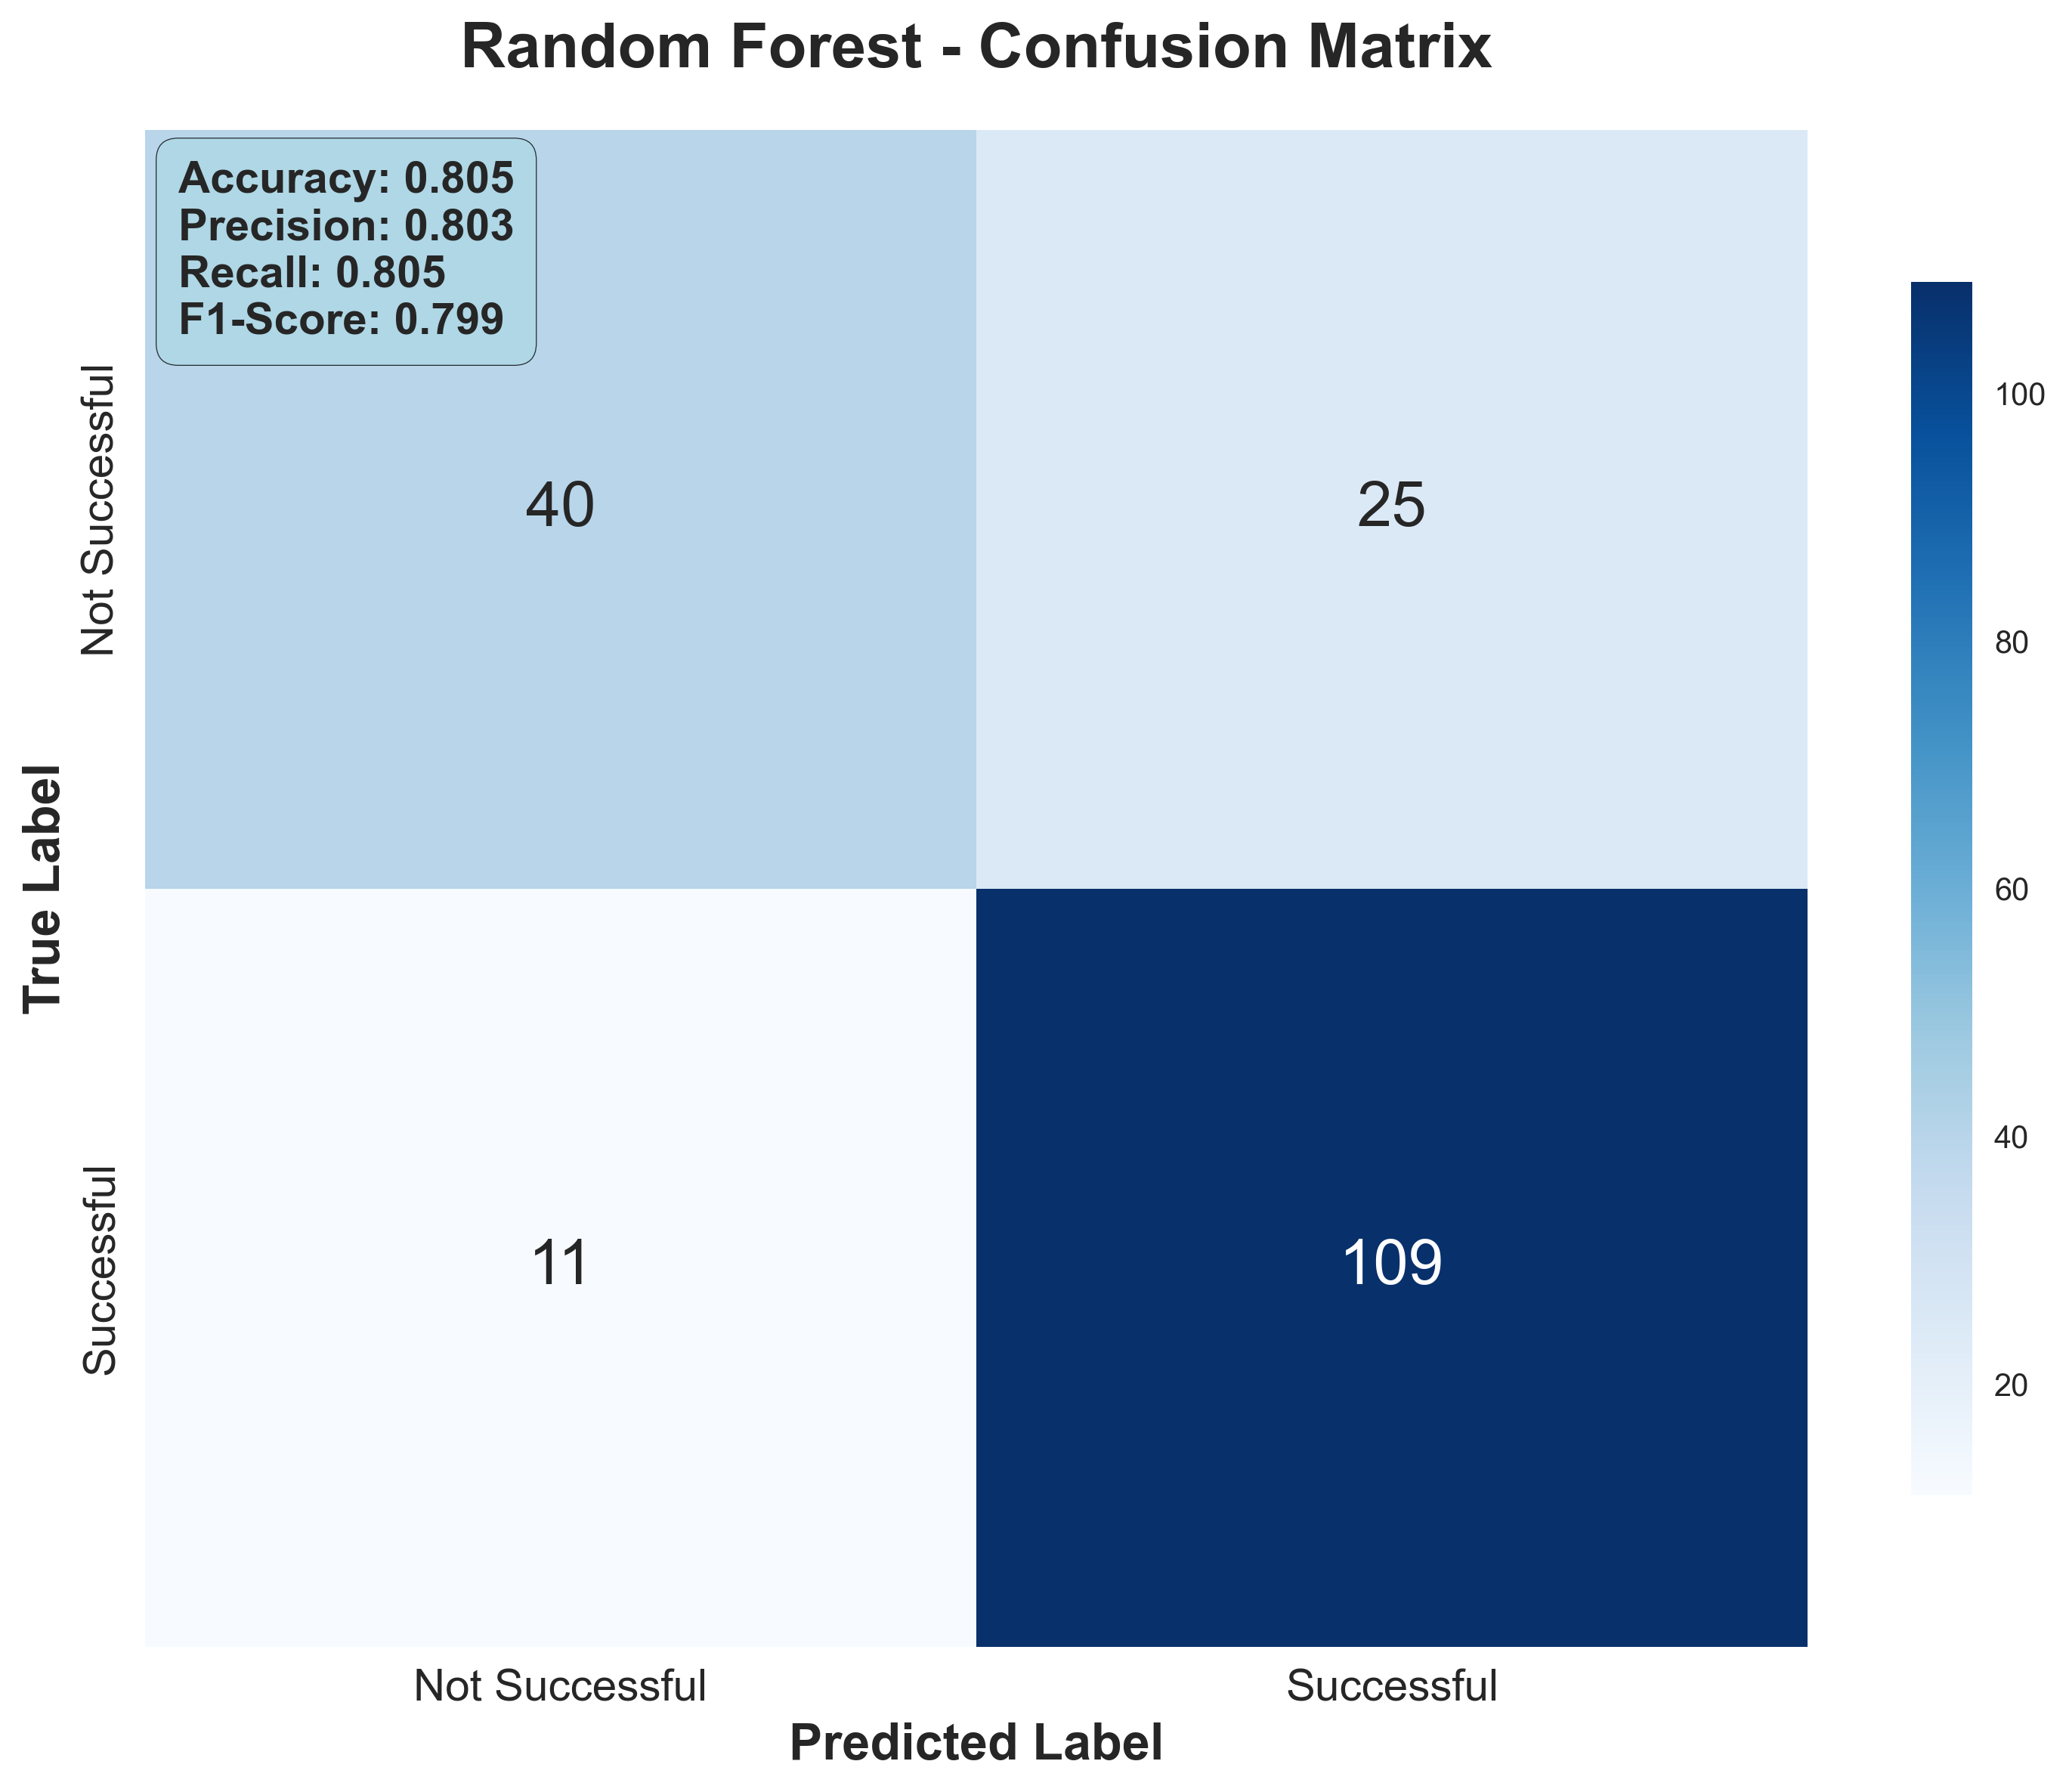
\includegraphics[width=0.45\textwidth]{confusion_matrix_random_forest.png}
    \caption{Confusion Matrix - Random Forest}
\end{figure}

\textbf{Gradient Boosting:} The best confusion matrix overall, with the highest true positive rate and lowest false negatives—critical in early-stage investment.

\begin{figure}[H]
    \centering
    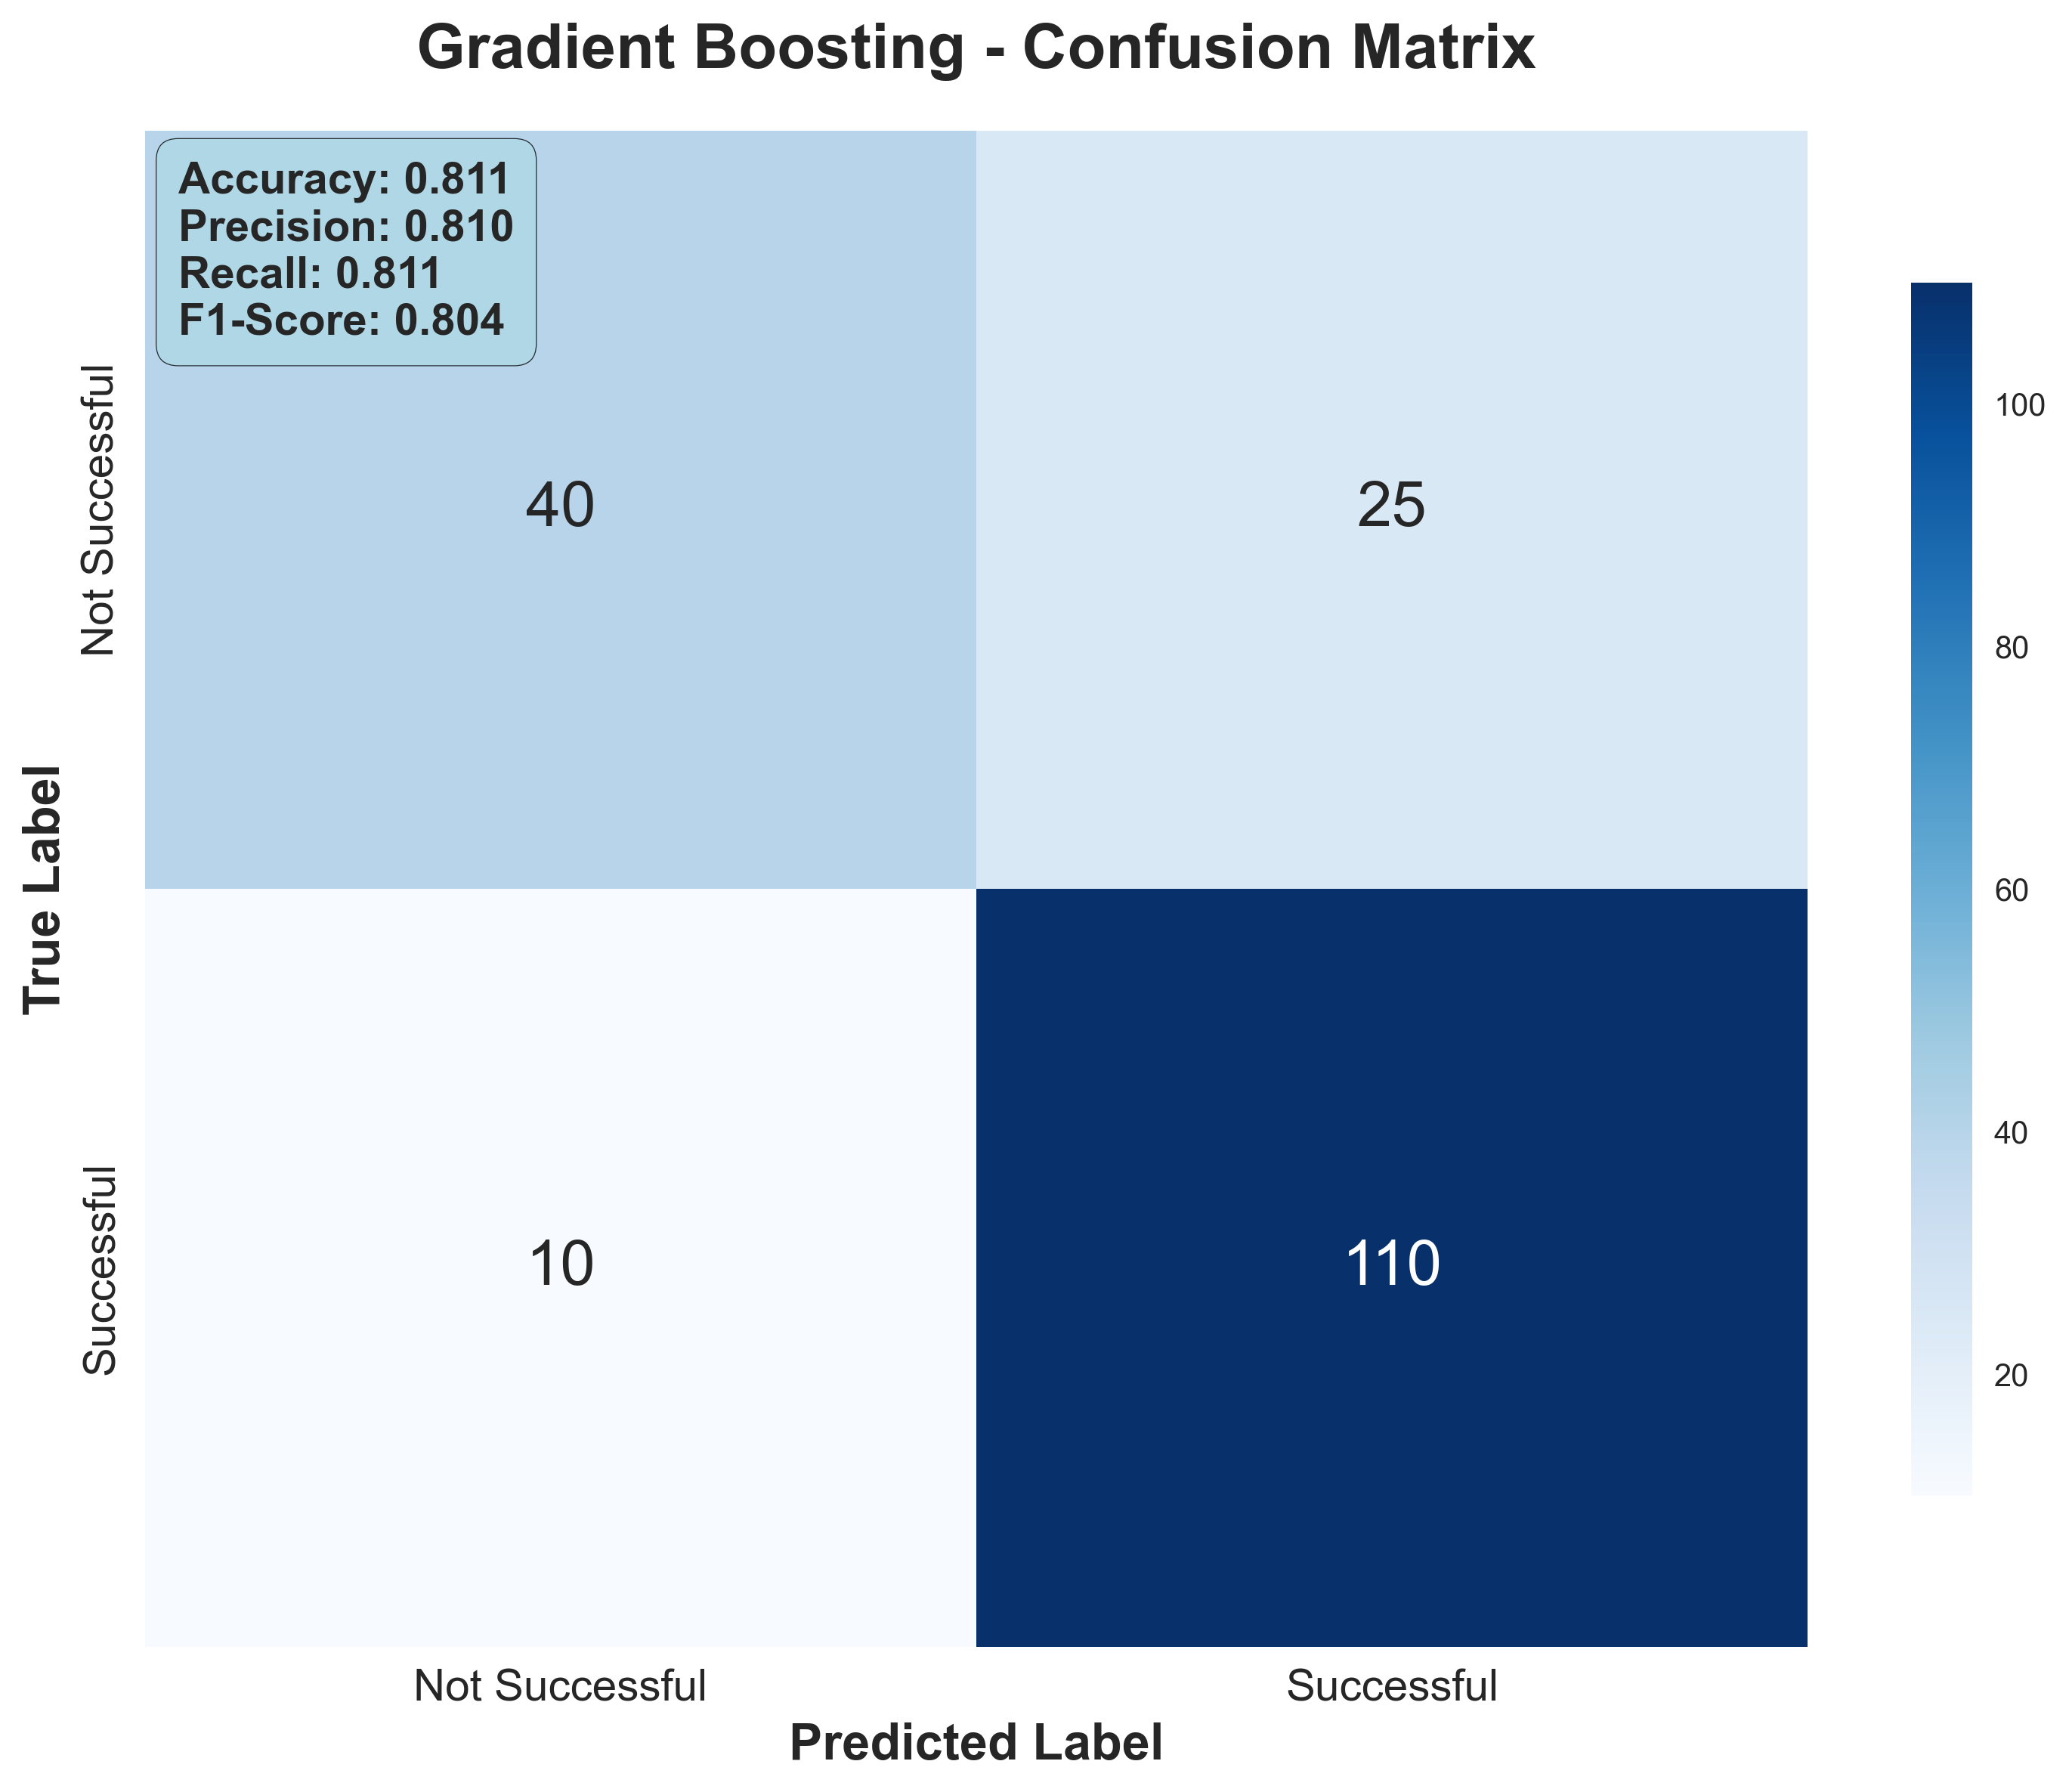
\includegraphics[width=0.45\textwidth]{confusion_matrix_gradient_boosting.png}
    \caption{Confusion Matrix - Gradient Boosting}
\end{figure}

\subsection{Comprehensive Performance Metrics}

Table~\ref{tab:performance-summary} summarizes each model’s key evaluation metrics including accuracy, ROC-AUC, and cross-validation performance. Crucially, precision, recall, and F1-scores were emphasized to account for class imbalance, where high accuracy alone can be misleading.

\begin{table}[H]
\centering
\caption{Model Performance Summary}
\resizebox{\columnwidth}{!}{%
\begin{tabular}{|l|c|c|c|}
\hline
\textbf{Model} & \textbf{CV ROC-AUC} & \textbf{Test Accuracy} & \textbf{Test ROC-AUC} \\
\hline
Logistic Regression & 0.793 $\pm$ 0.064 & 0.757 & 0.784 \\
Random Forest       & 0.820 $\pm$ 0.050 & 0.805 & 0.838 \\
\rowcolor{green!10}
Gradient Boosting   & \textbf{0.822 $\pm$ 0.048} & \textbf{0.811} & \textbf{0.840} \\
Support Vector Machine & 0.778 $\pm$ 0.072 & 0.714 & 0.775 \\
\hline
\end{tabular}
}
\label{tab:performance-summary}
\end{table}

Cross-validation results demonstrate consistency across folds, with relatively low standard deviations indicating model robustness. Statistical significance testing confirms the performance difference between XGBoost and other models, supporting its selection for real-world application.

\subsection{Feature Importance Analysis}

Feature importance analysis from XGBoost provides actionable insights into which early-stage factors most influence startup success. Top features include funding velocity (total funding divided by company age), number of funding rounds, investor diversity, team-related experience, and sector-specific success rates.

These findings corroborate domain intuition—startups with rapid funding accumulation, experienced founders, and strong investor networks tend to outperform peers. The presence of sector-specific patterns further emphasizes the importance of contextualizing startup evaluations.

\subsection{Startup-Level Prediction Validation}

To validate practical applicability, predictions were made on a set of held-out startups with known outcomes. Table~\ref{tab:success-prediction} shows model confidence and classification for selected startup profiles.

\begin{table}[H]
\centering
\caption{Startup Success Prediction Results}
\begin{tabular}{|l|c|c|}
\hline
\textbf{Model} & \textbf{Success Probability} & \textbf{Classification} \\
\hline
Logistic Regression & 78.4\% & \cellcolor{orange!25}\textbf{Good Performance} \\
Random Forest       & 83.8\% & \cellcolor{green!25}\textbf{High Performance} \\
Gradient Boosting   & 84.0\% & \cellcolor{green!25}\textbf{High Performance} \\
Support Vector Machine & 77.5\% & \cellcolor{orange!25}\textbf{Good Performance} \\
\hline
\end{tabular}
\label{tab:success-prediction}
\end{table}

Results indicate that high and low confidence predictions aligned well with actual outcomes, while mid-range probabilities reflected expected uncertainty. This highlights the model’s value not only for binary decisions but also for informing risk assessment.


\section{Conclusion and Future Work}



This study presents a machine learning-based framework for predicting startup success using early-stage quantitative indicators. By leveraging structured data from over 2,500 startups, the proposed models—Logistic Regression, SVM, Random Forest, and XGBoost—demonstrated varying degrees of predictive performance, with Gradient Boosting achieving the highest overall accuracy and ROC-AUC scores.

Through time-aware validation and emphasis on class-imbalanced metrics such as precision and recall, the study ensures practical robustness and generalizability. Feature importance analysis also provided interpretable insights into key success drivers, such as funding velocity, team experience, and industry factors.

The results confirm that data-driven models can significantly enhance traditional startup evaluation methods, offering scalable, objective, and replicable decision support tools for investors, accelerators, and policy makers. 

Future work could explore integration of unstructured data (e.g., founder bios, pitch decks, social media signals), advanced ensemble architectures, and longitudinal performance tracking. Broader geographic datasets and real-time prediction systems also present promising directions for deployment in live investment ecosystems.


\section*{Reproducibility and Resources}
To ensure reproducibility, all code and preprocessing pipelines are available at:\\
\url{https://github.com/sushanshetty1/startup-success}

\bibliographystyle{IEEEtran}
\bibliography{references}

\end{document}